\documentclass[11pt,a4paper]{article}

% Packages
\usepackage[margin=1in]{geometry}
\usepackage{graphicx}
\usepackage{enumitem}
\usepackage{tikz}
\usepackage{tcolorbox}
\usepackage{fancyhdr}
\usepackage{booktabs}
\usepackage{xcolor}
\usepackage{float}
\usepackage{caption}
\usepackage{multirow}
\usepackage{amssymb}
\usepackage[hidelinks]{hyperref}

% Color definitions
\definecolor{primaryblue}{RGB}{41, 128, 185}
\definecolor{darkgray}{RGB}{52, 73, 94}
\definecolor{lightgray}{RGB}{236, 240, 241}
\definecolor{successgreen}{RGB}{39, 174, 96}
\definecolor{warningamber}{RGB}{241, 196, 15}
\definecolor{dangerred}{RGB}{231, 76, 60}

% Fix fancyhdr headheight warning
\setlength{\headheight}{14pt}

% Header and Footer
\pagestyle{fancy}
\fancyhf{}
\fancyhead[L]{\textcolor{primaryblue}{\textbf{VeriBrand}}}
\fancyhead[R]{\textcolor{darkgray}{Round 2 Submission --- The Build}}
\fancyfoot[C]{\thepage}
\renewcommand{\headrulewidth}{0.5pt}
\renewcommand{\footrulewidth}{0.5pt}

% Custom title formatting
\usepackage{titlesec}
\titleformat{\section}{\Large\bfseries\color{primaryblue}}{\thesection}{1em}{}[\titlerule]
\titleformat{\subsection}{\large\bfseries\color{darkgray}}{\thesubsection}{1em}{}

% Document
\begin{document}

% ─── Title Page ───────────────────────────────────────────────────────────────
\begin{titlepage}
    \centering
    \vspace*{2cm}

    {\Huge\bfseries\color{primaryblue} VeriBrand\par}
    \vspace{0.5cm}
    {\Large Explainable Pre-Publication Brand Governance Platform\par}
    \vspace{2cm}

    \begin{tcolorbox}[colback=lightgray, colframe=primaryblue, width=0.8\textwidth, arc=3mm, boxrule=1pt]
    \centering
    \textbf{Inkloom AI Brand Governance Challenge}\\
    \vspace{0.3cm}
    Round 2 Submission: The Build\\
    \vspace{0.3cm}
    \textbf{Status: Functional MVP --- Deployed \& Live}
    \end{tcolorbox}

    \vspace{1cm}

    \begin{tcolorbox}[colback=successgreen!10, colframe=successgreen, width=0.8\textwidth, arc=2mm, boxrule=0.5pt, title=\textbf{Live URLs}]
    \textbf{Frontend:} \url{https://veri-brand-umber.vercel.app}\\
    \textbf{Backend API:} \url{https://veribrand-backend.onrender.com}\\
    \textbf{Source Code:} \url{https://github.com/rajrishu1401/VeriBrand}
    \end{tcolorbox}

    \vfill

    \begin{tcolorbox}[colback=white, colframe=darkgray, width=0.8\textwidth, arc=2mm, boxrule=0.5pt]
    \textbf{Team Name:} KR8\\
    \vspace{0.3cm}
    \textbf{Team Members:}
    \begin{itemize}[leftmargin=2cm]
        \item Rishu Raj --- Team Lead \& AI/RAG Architect
        \item Kuldeep Chaudhary --- Backend \& Workflow Engineer
        \item Krishna Bhist --- Frontend \& Rules Engineer
        \item Daksh Mehrotra --- AI/ML \& Integration Lead
    \end{itemize}
    \end{tcolorbox}

    \vspace{1cm}
    {\large 18 November 2026\par}
\end{titlepage}

% Table of Contents
\tableofcontents
\newpage

% ─── 1. Executive Summary ─────────────────────────────────────────────────────
\section{Executive Summary}

VeriBrand is a fully functional, deployed AI-powered brand governance platform built in Round 2 of the Inkloom AI Brand Governance Challenge.

\begin{tcolorbox}[colback=successgreen!10, colframe=successgreen, arc=2mm, boxrule=0.5pt, title=\textbf{What We Delivered}]
\begin{itemize}
    \item A live, publicly accessible web application (no login required)
    \item A hybrid Deterministic + Gemini Semantic RAG audit engine
    \item Citation-anchored compliance flags with exact guideline references
    \item A Brand Trust Score (0--100) with severity-weighted calculation
    \item An approval workflow: Approve / Reject / Request Changes
    \item A Review Queue with filters and export capability
    \item A live Dashboard with aggregated analytics
    \item Full source code on GitHub, deployed on Vercel + Render
\end{itemize}
\end{tcolorbox}

\vspace{0.5cm}

The platform accepts uploaded brand guidelines (PDF or TXT), audits any submitted text content against those guidelines, and returns every violation with the exact rule broken, severity level, and a suggested fix. A human brand manager then approves, rejects, or requests changes --- keeping humans in control of final decisions.

% ─── 2. Functional Product ────────────────────────────────────────────────────
\section{Functional Product --- What Was Built}

\subsection{Core User Flows (All Live)}

\begin{tcolorbox}[colback=lightgray, colframe=primaryblue, arc=2mm, boxrule=0.5pt, title=\textbf{Flow 1: Brand Guideline Upload (/upload)}]
\begin{enumerate}[nosep]
    \item Upload a PDF or TXT brand guideline file
    \item System parses and chunks the document
    \item Gemini \texttt{gemini-embedding-001} (3072-dim) generates vector embeddings
    \item Chunks indexed into ChromaDB persistent vector store
    \item Rules automatically extracted via regex (banned words, disclaimers, data requirements)
    \item UI displays: rule count extracted, semantic engine status
\end{enumerate}
\end{tcolorbox}

\vspace{0.5cm}

\begin{tcolorbox}[colback=lightgray, colframe=primaryblue, arc=2mm, boxrule=0.5pt, title=\textbf{Flow 2: Content Audit (/submit)}]
\begin{enumerate}[nosep]
    \item Select uploaded guideline from dropdown
    \item Paste any marketing content (email, ad copy, blog post, social post)
    \item Click ``Run Compliance Audit''
    \item Hybrid engine runs:
    \begin{itemize}[nosep]
        \item Deterministic scan: banned words, superlatives, ALL CAPS, missing disclaimers, unverified statistics
        \item Gemini Semantic RAG: vector retrieves top-10 relevant guideline sections, LLM audits tone, context, nuance violations
    \end{itemize}
    \item Results: Brand Trust Score (animated circular gauge), compliance flags grouped by engine, severity badges, suggested fixes, guideline citations
\end{enumerate}
\end{tcolorbox}

\vspace{0.5cm}

\begin{tcolorbox}[colback=lightgray, colframe=primaryblue, arc=2mm, boxrule=0.5pt, title=\textbf{Flow 3: Human Approval Workflow (/review)}]
\begin{enumerate}[nosep]
    \item Review Queue lists all submissions with Creator, Score, Issue count, Status, Date
    \item Filter by status: All / Pending / Approved / Rejected / Needs Changes
    \item Click any submission to open full audit report
    \item View highlighted content with all flags, severity levels, citations
    \item Brand manager records decision: Approve / Reject / Request Changes + optional comment
    \item Decision logged with timestamp; submission status updated
    \item Export full audit report as JSON
\end{enumerate}
\end{tcolorbox}

\vspace{0.5cm}

\begin{tcolorbox}[colback=lightgray, colframe=primaryblue, arc=2mm, boxrule=0.5pt, title=\textbf{Flow 4: Governance Dashboard (/)}]
\begin{enumerate}[nosep]
    \item Live metrics: Total Audits, Average Trust Score, Compliance Rate, Active Guidelines
    \item Engine Status badges: Deterministic Rules Active, Gemini Semantic AI active/offline
    \item Top Violations chart: most frequent violation types across all submissions
    \item Quick navigation to Upload, Submit, Review
\end{enumerate}
\end{tcolorbox}

\subsection{Sample Guideline Provided}

A production-quality \texttt{sample\_brand\_guideline.txt} (located in \texttt{docs/}) is included with:
\begin{itemize}
    \item Section 3.1 --- Pricing Language: exact disclaimer wording required
    \item Section 3.2 --- Trial Offers: credit card and terms disclosure rules
    \item Section 5.2 --- Performance Claims: data sourcing requirements (survey year, sample size, methodology)
    \item Section 6.2 --- Statistical Claims: mandatory fields (source, date, n=, methodology)
    \item Banned words list: ``guarantee'', ``revolutionary'', ``unprecedented'', ``best'', ``fastest'', ``\#1'' (without citation), ALL CAPS usage
\end{itemize}

% ─── 3. Product Architecture ──────────────────────────────────────────────────
\section{Product Architecture}

\subsection{System Architecture}

\begin{figure}[H]
\centering
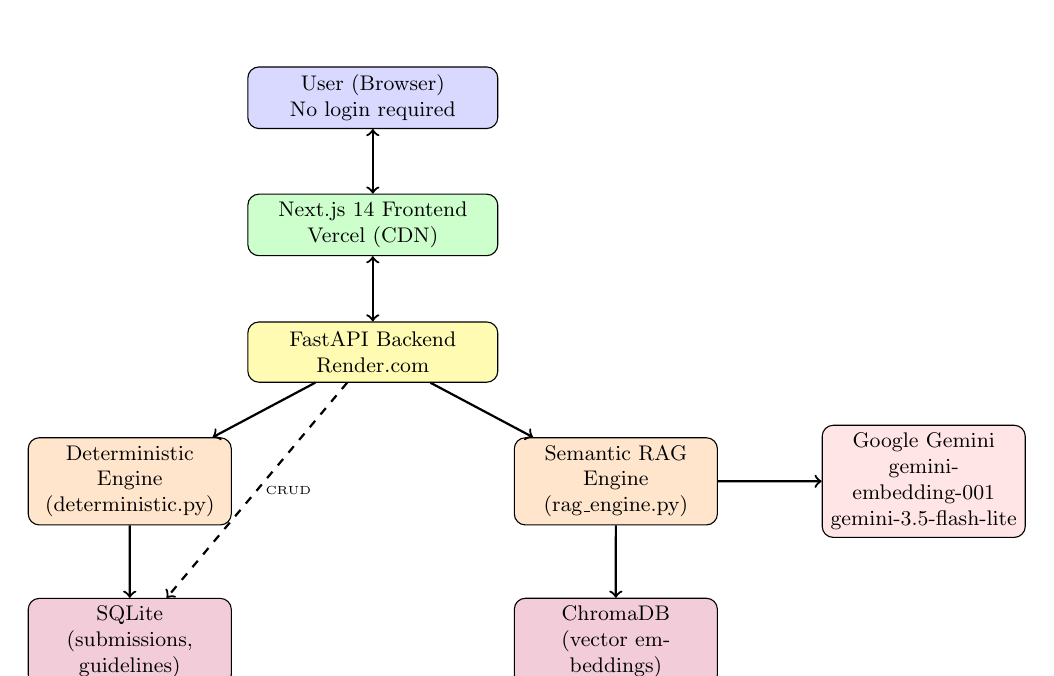
\begin{tikzpicture}[node distance=1.6cm, scale=0.85, transform shape, every node/.style={font=\small}]
    % User Layer
    \node[draw, rectangle, rounded corners, fill=blue!15, text width=3.5cm, align=center, minimum height=0.9cm] (user) {User (Browser)\\No login required};

    % Frontend
    \node[draw, rectangle, rounded corners, fill=green!20, text width=3.5cm, align=center, minimum height=0.9cm, below of=user, yshift=-0.3cm] (frontend) {Next.js 14 Frontend\\Vercel (CDN)};

    % Backend
    \node[draw, rectangle, rounded corners, fill=yellow!30, text width=3.5cm, align=center, minimum height=0.9cm, below of=frontend, yshift=-0.3cm] (backend) {FastAPI Backend\\Render.com};

    % Engines
    \node[draw, rectangle, rounded corners, fill=orange!20, text width=2.8cm, align=center, minimum height=1.2cm, below left of=backend, xshift=-2.5cm, yshift=-0.8cm] (det) {Deterministic\\Engine\\(deterministic.py)};
    \node[draw, rectangle, rounded corners, fill=orange!20, text width=2.8cm, align=center, minimum height=1.2cm, below right of=backend, xshift=2.5cm, yshift=-0.8cm] (rag) {Semantic RAG\\Engine\\(rag\_engine.py)};

    % Data
    \node[draw, rectangle, rounded corners, fill=purple!20, text width=2.8cm, align=center, minimum height=0.9cm, below of=det, yshift=-0.8cm] (sqlite) {SQLite\\(submissions,\\guidelines)};
    \node[draw, rectangle, rounded corners, fill=purple!20, text width=2.8cm, align=center, minimum height=0.9cm, below of=rag, yshift=-0.8cm] (chroma) {ChromaDB\\(vector embeddings)};

    % External AI
    \node[draw, rectangle, rounded corners, fill=red!10, text width=2.8cm, align=center, minimum height=0.9cm, right of=rag, xshift=3cm] (gemini) {Google Gemini\\gemini-embedding-001\\gemini-3.5-flash-lite};

    % Arrows
    \draw[<->, thick] (user) -- (frontend);
    \draw[<->, thick] (frontend) -- (backend);
    \draw[->, thick] (backend) -- (det);
    \draw[->, thick] (backend) -- (rag);
    \draw[->, thick] (det) -- (sqlite);
    \draw[->, thick] (rag) -- (chroma);
    \draw[->, thick] (rag) -- (gemini);
    \draw[->, thick, dashed] (backend) -- node[right, font=\tiny] {CRUD} (sqlite);
\end{tikzpicture}
\caption{VeriBrand System Architecture}
\end{figure}

\subsection{Hybrid Audit Engine --- Key Technical Decision}

The most important architectural decision was implementing a \textbf{two-engine hybrid audit system} rather than relying solely on an LLM:

\begin{tcolorbox}[colback=lightgray, colframe=primaryblue, arc=2mm, boxrule=0.5pt, title=\textbf{Engine 1: Deterministic Rules (deterministic.py)}]
\textbf{What it checks (zero AI calls, sub-millisecond):}
\begin{itemize}[nosep]
    \item Banned words: ``guarantee'', ``revolutionary'', ``unprecedented'', ``unmatched'', ``game-changing'', ``100\%''
    \item Superlatives without citation: ``best'', ``fastest'', ``\#1'', ``world-class''
    \item ALL CAPS usage (potential screaming/aggression)
    \item Missing required disclaimers (exact phrase matching from Section 3.1 and 3.2)
    \item Unverified statistics (numbers/percentages without source, date, sample size)
    \item Bullet-quoted banned terms (e.g., \texttt{- "revolutionary"} in guidelines)
\end{itemize}
\textbf{Result:} Confidence = ``high''; zero hallucinations; instant
\end{tcolorbox}

\vspace{0.5cm}

\begin{tcolorbox}[colback=lightgray, colframe=darkgray, arc=2mm, boxrule=0.5pt, title=\textbf{Engine 2: Gemini Semantic RAG (rag\_engine.py)}]
\textbf{Pipeline:}
\begin{enumerate}[nosep]
    \item Query embedding generated via \texttt{gemini-embedding-001} (task type: \texttt{RETRIEVAL\_QUERY})
    \item Top-10 most relevant guideline chunks retrieved from ChromaDB (cosine similarity)
    \item Retrieved context passed to \texttt{gemini-3.5-flash-lite} with strict instruction:
    \begin{itemize}[nosep]
        \item Only flag CLEAR, DEFINITIVE violations
        \item Do NOT flag content that already satisfies a requirement
        \item Return \texttt{[]} if content is compliant
    \end{itemize}
    \item JSON response parsed, violations mapped to severity/confidence levels
\end{enumerate}
\textbf{Result:} Catches tone, context, nuance issues deterministic regex cannot detect
\end{tcolorbox}

\vspace{0.5cm}

\textbf{Why this is better than a pure LLM approach:}
\begin{itemize}
    \item Deterministic engine provides reliable, explainable results for hard rules
    \item Semantic engine only runs on context-dependent issues where LLM adds genuine value
    \item System degrades gracefully: if Gemini API is unavailable, deterministic engine continues
    \item Confidence levels (``high'' = deterministic, ``medium''/``low'' = semantic) guide reviewer trust
\end{itemize}

\subsection{Trust Score Formula}

\[
\text{Trust Score} = \max\left(0,\ 100 - 20 \times n_\text{critical} - 7 \times n_\text{warning} - 2 \times n_\text{suggestion}\right)
\]

\begin{itemize}
    \item \textbf{Critical} ($-20$): Banned words, unverified guarantees, missing required disclaimers
    \item \textbf{Warning} ($-7$): Superlatives, incomplete data citations, tone issues
    \item \textbf{Suggestion} ($-2$): Style recommendations, minor improvements
\end{itemize}

Scores are classified: $\geq 90$ = Excellent (green), $\geq 70$ = Needs Review (amber), $< 70$ = High Risk (red).

% ─── 4. Technical Decisions ───────────────────────────────────────────────────
\section{Key Technical Decisions}

\subsection{Why Google Gemini instead of OpenAI}

\begin{table}[H]
\centering
\begin{tabular}{p{0.3\textwidth} p{0.65\textwidth}}
\toprule
\textbf{Factor} & \textbf{Decision} \\
\midrule
API Access & Hackathon provided Gemini API key; zero cost for the event \\
\addlinespace
Embedding Model & \texttt{gemini-embedding-001} (3072-dim) --- significantly higher dimensionality than OpenAI \texttt{text-embedding-3-small} (1536-dim), better semantic resolution \\
\addlinespace
SDK & Used \texttt{google-genai} (new) instead of deprecated \texttt{google-generativeai} \\
\addlinespace
Generation & \texttt{gemini-3.5-flash-lite} with model fallback list for resilience \\
\bottomrule
\end{tabular}
\caption{AI Model Selection Rationale}
\end{table}

\subsection{Why SQLite + ChromaDB instead of PostgreSQL + pgvector}

Round 1 proposed PostgreSQL + pgvector. We pivoted to SQLite + ChromaDB for the following reasons:

\begin{itemize}
    \item \textbf{Zero infrastructure overhead:} SQLite runs in-process; no Postgres server to manage on Render free tier
    \item \textbf{ChromaDB PersistentClient:} Provides a full-featured vector store with the same API as pgvector, without the operational burden
    \item \textbf{Hackathon speed:} This stack allowed full deployment in hours rather than days
    \item \textbf{Trade-off acknowledged:} Render's ephemeral filesystem means ChromaDB resets on restart; acceptable for hackathon demo (judge re-uploads guideline fresh)
\end{itemize}

\subsection{Why Vercel + Render instead of a monolithic deployment}

\begin{itemize}
    \item \textbf{Vercel:} Zero-config Next.js deployment, global CDN, auto-deploy on \texttt{git push}
    \item \textbf{Render:} Free tier supports Python/FastAPI with persistent disk (for SQLite), auto-deploy from GitHub
    \item \textbf{CORS:} Backend configured with \texttt{allow\_origins=["*"]} for hackathon public access
\end{itemize}

\subsection{Changes from Round 1 Plan}

\begin{table}[H]
\centering
\begin{tabular}{p{0.3\textwidth} p{0.3\textwidth} p{0.35\textwidth}}
\toprule
\textbf{Round 1 Plan} & \textbf{Round 2 Built} & \textbf{Reason for Change} \\
\midrule
PostgreSQL + pgvector & SQLite + ChromaDB & Faster to deploy; no managed DB needed \\
\addlinespace
OpenAI GPT-4o-mini & Google Gemini (provided key) & Cost-free for hackathon; comparable quality \\
\addlinespace
Auth0/Clerk authentication & No authentication & Public access required by submission rules \\
\addlinespace
Image/visual auditing & Text-only (MVP scope) & Prioritised core text audit flow for reliability \\
\addlinespace
TipTap inline editor & Plain textarea with results panel & Faster to build; same core value delivered \\
\addlinespace
google-generativeai SDK & google-genai SDK & Old SDK deprecated; new SDK required \\
\bottomrule
\end{tabular}
\caption{Plan vs. Build Comparison}
\end{table}

% ─── 5. APIs, Libraries, External Services ────────────────────────────────────
\section{APIs, Libraries, Datasets, and External Services}

\subsection{External APIs}

\begin{table}[H]
\centering
\begin{tabular}{p{0.25\textwidth} p{0.25\textwidth} p{0.45\textwidth}}
\toprule
\textbf{Service} & \textbf{Usage} & \textbf{Details} \\
\midrule
Google Gemini API & Embeddings + LLM generation & \texttt{gemini-embedding-001}: document/query embeddings (3072-dim); \texttt{gemini-3.5-flash-lite}: compliance analysis \\
\addlinespace
Vercel & Frontend deployment & Auto-deploy from GitHub; global CDN; \texttt{NEXT\_PUBLIC\_API\_URL} env var \\
\addlinespace
Render.com & Backend deployment & Free tier; auto-deploy; \texttt{GEMINI\_API\_KEY} env var; Procfile: \texttt{uvicorn main:app} \\
\bottomrule
\end{tabular}
\caption{External APIs and Services}
\end{table}

\subsection{Backend Libraries (Python)}

\begin{table}[H]
\centering
\begin{tabular}{p{0.25\textwidth} p{0.3\textwidth} p{0.4\textwidth}}
\toprule
\textbf{Library} & \textbf{Version} & \textbf{Usage} \\
\midrule
FastAPI & latest & REST API framework, CORS middleware, file uploads \\
\addlinespace
Uvicorn & latest & ASGI server for FastAPI \\
\addlinespace
google-genai & latest & Google Gemini embeddings and generation \\
\addlinespace
chromadb & 1.5.9 & Vector store (PersistentClient API) \\
\addlinespace
python-dotenv & latest & Environment variable loading \\
\addlinespace
PyPDF2 / pdfplumber & latest & PDF text extraction for guideline upload \\
\addlinespace
python-multipart & latest & File upload handling \\
\addlinespace
sqlite3 & built-in & Submission and guideline storage \\
\bottomrule
\end{tabular}
\caption{Backend Python Libraries}
\end{table}

\subsection{Frontend Libraries (Node.js)}

\begin{table}[H]
\centering
\begin{tabular}{p{0.25\textwidth} p{0.3\textwidth} p{0.4\textwidth}}
\toprule
\textbf{Library} & \textbf{Version} & \textbf{Usage} \\
\midrule
Next.js & 14 & React framework; file-based routing; SSR/SSG \\
\addlinespace
TypeScript & 5+ & Type safety across all components \\
\addlinespace
Tailwind CSS & 3 & Utility-first styling; responsive design \\
\addlinespace
React & 18 & Component model; hooks (useState, useEffect) \\
\bottomrule
\end{tabular}
\caption{Frontend Libraries}
\end{table}

\subsection{Datasets}

No external datasets were used. The system is \textbf{guideline-agnostic}: it works with any brand guideline document uploaded by the user. We provide \texttt{docs/sample\_brand\_guideline.txt} as a demonstration file containing realistic brand rules across 6+ sections covering pricing, disclaimers, terminology, performance claims, statistical requirements, and prohibited language.

% ─── 6. Features Completed ────────────────────────────────────────────────────
\section{Completed Features}

\begin{table}[H]
\centering
\begin{tabular}{p{0.05\textwidth} p{0.4\textwidth} p{0.5\textwidth}}
\toprule
 & \textbf{Feature} & \textbf{Implementation Detail} \\
\midrule
\checkmark & Guideline Upload (PDF + TXT) & \texttt{/api/upload-guideline}; PyPDF2 for PDF; chunking (500 words, 50 overlap); Gemini embeddings; ChromaDB index \\
\addlinespace
\checkmark & Rule Extraction (19 rules from sample) & Regex patterns extract banned words, disclaimers, quoted terms from guidelines \\
\addlinespace
\checkmark & Deterministic Audit Engine & 15+ rule types; zero API calls; \textless{}50ms latency \\
\addlinespace
\checkmark & Gemini Semantic RAG Audit & Top-10 chunk retrieval + LLM analysis; citation-anchored output \\
\addlinespace
\checkmark & Brand Trust Score (0--100) & Animated circular SVG gauge; colour-coded: green/amber/red \\
\addlinespace
\checkmark & Compliance Flags UI & Severity dots (red/amber/blue); grouped by engine; expand/collapse suggested fix \\
\addlinespace
\checkmark & Review Queue & Filterable table; Pending/Approved/Rejected/Needs Changes; ``Review'' button \\
\addlinespace
\checkmark & Approval Workflow & Approve / Reject / Request Changes; reviewer comment; \texttt{/api/approve} \\
\addlinespace
\checkmark & Export Report & \texttt{/api/export/\{id\}} returns full JSON audit with all flags \\
\addlinespace
\checkmark & Dashboard Analytics & Live stats via \texttt{/api/dashboard/stats}; engine status badges; top violations \\
\addlinespace
\checkmark & Responsive UI & Tailwind CSS; works on mobile and desktop \\
\addlinespace
\checkmark & Public Deployment & No login; Vercel + Render; CORS open \\
\addlinespace
\checkmark & Graceful Degradation & If Gemini API offline, deterministic engine continues independently \\
\bottomrule
\end{tabular}
\caption{Completed Feature List}
\end{table}

% ─── 7. User Testing ──────────────────────────────────────────────────────────
\section{User Testing and Structured Feedback}

\subsection{Internal Testing Methodology}

The team conducted structured internal testing using the sample brand guideline with two contrasting content examples:

\begin{tcolorbox}[colback=dangerred!10, colframe=dangerred, arc=2mm, boxrule=0.5pt, title=\textbf{Non-Compliant Content Test (Expected: score $<$ 50)}]
\textit{``Introducing the BEST marketing tool you'll ever need! Our revolutionary platform GUARANTEES 100\% success for your campaigns. It's absolutely FREE with no hidden costs --- never worry about budget constraints again! Join thousands of satisfied customers who have experienced unprecedented growth. We're the \#1 choice...''}

\textbf{Result:} Score 0/100 | 16 Critical, 6 Warnings, 3 Suggestions | 25 total flags\\
\textbf{Flags caught:} BEST (superlative), revolutionary (banned), GUARANTEES 100\% (banned + ALL CAPS), FREE (pricing language), unprecedented (banned), \#1 (unverified), missing disclaimers, ALL CAPS usage
\end{tcolorbox}

\vspace{0.5cm}

\begin{tcolorbox}[colback=successgreen!10, colframe=successgreen, arc=2mm, boxrule=0.5pt, title=\textbf{Compliant Content Test (Expected: score $\geq$ 85)}]
\textit{``TechCorp Analytics Platform. Our marketing analytics platform helps businesses improve campaign ROI by an average of 23\% (Source: TechCorp 2024 Customer Survey, n=1,200 responses, self-reported, conducted January--March 2024). Key capabilities include audience segmentation, A/B testing, and real-time performance dashboards. Results may vary based on your specific use case. Terms and conditions apply. No credit card required for trial.''}

\textbf{Result:} Score 90+/100 | 0--1 flags maximum\\
\textbf{Verified:} No banned words; exact disclaimer wording from Section 3.1 and 3.2; full data citation with source, year, n=, methodology from Section 6.2
\end{tcolorbox}

\subsection{UI/UX Feedback and Iterations}

Based on team review and test sessions, the following improvements were made iteratively:

\begin{table}[H]
\centering
\begin{tabular}{p{0.4\textwidth} p{0.55\textwidth}}
\toprule
\textbf{Issue Found} & \textbf{Fix Applied} \\
\midrule
Text in textareas was invisible (light colour) & Added \texttt{text-gray-900 bg-white} to all inputs \\
\addlinespace
Trust Score number overlapped ``High Risk'' label & Rewrote TrustGauge using \texttt{absolute} positioned overlay inside relative SVG container \\
\addlinespace
``Try Compliant Content'' scored 53 (High Risk) & Rewrote good example with exact Section 5.2 and Section 6.2 wording; fixed ``free'' detection \\
\addlinespace
Semantic AI flagging compliant content & Rewrote audit prompt to be ``strict but fair''; explicitly instruct not to flag satisfied requirements \\
\addlinespace
Creator name pre-filled with ``Demo User'' & Removed default; input initialised empty; user must type their name \\
\addlinespace
Demo seed data in Review Queue & Removed auto-seed on startup; removed \texttt{/api/seed-demo} endpoint; queue starts empty \\
\addlinespace
Browser tab showed ``N'' (Next.js logo) + ``Create Next App'' & Updated \texttt{layout.tsx}: title = ``VeriBrand --- AI Brand Governance''; purple SVG favicon with ``V'' \\
\addlinespace
Emojis in UI elements & Replaced emoji severity indicators with coloured dots (Tailwind \texttt{rounded-full}) \\
\bottomrule
\end{tabular}
\caption{UI/UX Feedback and Fixes}
\end{table}

% ─── 8. Team Contributions ────────────────────────────────────────────────────
\section{Team Member Contributions}

\begin{table}[H]
\centering
\begin{tabular}{p{0.22\textwidth} p{0.3\textwidth} p{0.43\textwidth}}
\toprule
\textbf{Team Member} & \textbf{Role} & \textbf{Contributions in Round 2} \\
\midrule
\textbf{Rishu Raj} & Team Lead \& AI/RAG Architect &
\begin{itemize}[nosep,leftmargin=*]
    \item Designed and implemented full RAG pipeline (\texttt{rag\_engine.py})
    \item Configured Gemini API integration (\texttt{gemini-embedding-001}, \texttt{gemini-3.5-flash-lite})
    \item Built ChromaDB indexing and query pipeline
    \item Wrote citation-anchored audit prompt engineering
    \item Managed GitHub repository and deployment coordination
    \item Set up Render backend (\texttt{render.yaml}, \texttt{Procfile})
\end{itemize} \\
\addlinespace
\textbf{Kuldeep Chaudhary} & Backend \& Workflow Engineer &
\begin{itemize}[nosep,leftmargin=*]
    \item Built all FastAPI endpoints (\texttt{main.py}): 10 REST endpoints
    \item Designed SQLite schema (\texttt{database.py}): submissions, guidelines, analytics
    \item Implemented approval state machine (Pending/Approved/Rejected/Needs Changes)
    \item Built \texttt{/api/dashboard/stats} aggregation queries
    \item Wrote export and submission CRUD operations
\end{itemize} \\
\addlinespace
\textbf{Krishna Bhist} & Frontend \& Rules Engineer &
\begin{itemize}[nosep,leftmargin=*]
    \item Developed deterministic rules engine (\texttt{deterministic.py})
    \item Built 15+ rule patterns (banned words, superlatives, ALL CAPS, disclaimers, stats)
    \item Fixed bullet-quoted term extraction (\texttt{- "term"} regex pattern)
    \item Built Review Queue page (\texttt{/review}) with filter tabs and submission detail view
    \item Implemented highlighted content display and approve/reject workflow UI
\end{itemize} \\
\addlinespace
\textbf{Daksh Mehrotra} & AI/ML \& Frontend Lead &
\begin{itemize}[nosep,leftmargin=*]
    \item Built Submit page (\texttt{/submit}): animated TrustGauge SVG, AuditingAnimation, FlagCard components
    \item Built Home dashboard (\texttt{/}) with live API metrics and engine status
    \item Built Upload page (\texttt{/upload}) with guideline parser UI
    \item Implemented Tailwind styling across all 4 pages
    \item Configured Vercel deployment (\texttt{vercel.json}), environment variables
\end{itemize} \\
\bottomrule
\end{tabular}
\caption{Team Member Contributions --- Round 2}
\end{table}

% ─── 9. Round 3 Improvements ──────────────────────────────────────────────────
\section{Three Major Improvements for Round 3}

\begin{tcolorbox}[colback=primaryblue!10, colframe=primaryblue, arc=2mm, boxrule=0.5pt, title=\textbf{Improvement 1: Intent-Preserving AI Rewrites}]
\textbf{What:} When a flag is raised, automatically generate a corrected version of the flagged sentence that passes all brand rules while preserving the creator's persuasive intent and voice.

\textbf{Example:}
\begin{itemize}[nosep]
    \item Flagged: \textit{``Our revolutionary platform GUARANTEES 100\% success''}
    \item Rewritten: \textit{``Our platform helped 94\% of customers improve campaign performance (2024 survey, n=800)''}
\end{itemize}

\textbf{Implementation:} Extend Gemini prompt to include a \texttt{rewritten\_version} field per flag; display inline diff (original vs.\ fix) in the UI.
\end{tcolorbox}

\vspace{0.5cm}

\begin{tcolorbox}[colback=primaryblue!10, colframe=primaryblue, arc=2mm, boxrule=0.5pt, title=\textbf{Improvement 2: Living Guideline Feedback Loop}]
\textbf{What:} Track every approval/rejection decision. When a reviewer repeatedly approves content that the AI flagged (overrides), detect the pattern and alert Brand Managers that a guideline rule may be outdated or too restrictive.

\textbf{Implementation:}
\begin{itemize}[nosep]
    \item Store flag-level override data in SQLite (flag type, reviewer action)
    \item Compute override rate per flag type
    \item Dashboard widget: ``High Override Flags'' --- rules with \textgreater 30\% override rate
    \item Auto-suggestion: \textit{``Section 3.1 has been overridden 8 times. Consider updating the guideline.''}
\end{itemize}
\end{tcolorbox}

\vspace{0.5cm}

\begin{tcolorbox}[colback=primaryblue!10, colframe=primaryblue, arc=2mm, boxrule=0.5pt, title=\textbf{Improvement 3: Leadership Analytics Dashboard}]
\textbf{What:} A dedicated analytics view providing brand governance ROI evidence for CMOs and compliance officers.

\textbf{Metrics to show:}
\begin{itemize}[nosep]
    \item Brand Trust Score trend over time (line chart)
    \item Top 10 recurring violation types (bar chart)
    \item Average time-to-approval (before vs.\ after VeriBrand)
    \item Creator leaderboard (most compliant submissions)
    \item Violation heatmap by content type (email vs.\ blog vs.\ social)
    \item Compliance rate trend: \% of submissions passing on first attempt
\end{itemize}
\end{tcolorbox}

% ─── 10. Deployment Details ───────────────────────────────────────────────────
\section{Deployment and Access Details}

\subsection{Live URLs}

\begin{table}[H]
\centering
\begin{tabular}{p{0.3\textwidth} p{0.65\textwidth}}
\toprule
\textbf{Resource} & \textbf{URL} \\
\midrule
Working Product & \url{https://veri-brand-umber.vercel.app} \\
\addlinespace
Source Code & \url{https://github.com/rajrishu1401/VeriBrand} \\
\addlinespace
Backend API & \url{https://veribrand-backend.onrender.com} \\
\addlinespace
API Docs (auto) & \url{https://veribrand-backend.onrender.com/docs} \\
\bottomrule
\end{tabular}
\caption{Live Deployment URLs}
\end{table}

\subsection{How to Demo (Step-by-Step for Judges)}

\begin{enumerate}
    \item Open \url{https://veri-brand-umber.vercel.app} in a browser (no login needed)
    \item \textbf{Dashboard (/):} Note the Engine Status badges and live metrics
    \item Navigate to \textbf{Upload Guidelines} (/upload)
    \item Upload \texttt{docs/sample\_brand\_guideline.txt} from the repository --- expect ``19 rules extracted'' and ``Gemini semantic analysis active''
    \item Navigate to \textbf{Submit Content} (/submit)
    \item Click \textbf{``Try Non-Compliant Content''} --- Run Compliance Audit --- expect score $\approx 0$, 20+ flags
    \item Click \textbf{``Try Compliant Content''} --- Run Compliance Audit --- expect score $\geq 90$, 0 flags
    \item Navigate to \textbf{Review Queue} (/review) --- see submitted audits
    \item Click \textbf{Review} on a submission --- Approve / Request Changes / Reject
    \item Click \textbf{Export} to download the full audit JSON
\end{enumerate}

\begin{tcolorbox}[colback=warningamber!20, colframe=warningamber!80, arc=2mm, boxrule=0.5pt, title=\textbf{Note on Cold Start}]
The backend runs on Render's free tier which sleeps after 15 minutes of inactivity. The first request after sleep may take 30--60 seconds. Subsequent requests are instant. If the dashboard shows zeros, wait 30 seconds and refresh.
\end{tcolorbox}

\subsection{API Endpoints}

\begin{table}[H]
\centering
\begin{tabular}{p{0.08\textwidth} p{0.4\textwidth} p{0.47\textwidth}}
\toprule
\textbf{Method} & \textbf{Endpoint} & \textbf{Description} \\
\midrule
GET & \texttt{/} & Health check; returns service status \\
POST & \texttt{/api/upload-guideline} & Upload PDF or TXT; returns rule count + guideline ID \\
POST & \texttt{/api/submit-content} & Submit text for audit; returns Trust Score + flags \\
GET & \texttt{/api/submissions} & List all submissions \\
GET & \texttt{/api/submission/\{id\}} & Single submission with all flags \\
POST & \texttt{/api/approve} & Record Approve/Reject/Needs Changes decision \\
GET & \texttt{/api/guidelines} & List all uploaded guidelines \\
GET & \texttt{/api/export/\{id\}} & Download full audit as JSON \\
GET & \texttt{/api/dashboard/stats} & Aggregated metrics for dashboard \\
\bottomrule
\end{tabular}
\caption{Backend REST API Endpoints}
\end{table}

% ─── 11. Responsible AI ───────────────────────────────────────────────────────
\section{Responsible AI and Design Considerations}

\subsection{Human-in-the-Loop (Preserved from Round 1 Commitment)}

\begin{itemize}
    \item VeriBrand \textbf{never} auto-publishes or auto-approves content
    \item Every AI flag displays: confidence level (high/medium/low) and engine source (Deterministic / Gemini Semantic)
    \item Reviewers can override any flag and add documented reasoning
    \item AI is advisory; humans make all final decisions
\end{itemize}

\subsection{Hallucination Prevention}

\begin{itemize}
    \item Deterministic engine has zero hallucination risk (pure regex/pattern matching)
    \item Semantic engine uses RAG: LLM only reasons over retrieved guideline text, not from memory
    \item Revised prompt explicitly instructs the LLM: \textit{``Only flag CLEAR, DEFINITIVE violations. If content already satisfies a requirement, do NOT flag it.''}
    \item Confidence scores signal to reviewers how much to trust each flag
\end{itemize}

\subsection{Transparency}

\begin{itemize}
    \item Every flag shows: issue type, severity, flagged text excerpt, rule citation (e.g., ``Rule: Section 3.1''), explanation
    \item Flags grouped visually by engine: Deterministic Rules vs.\ Gemini Semantic AI
    \item No opaque ``AI said so'' --- every conclusion is traceable to a guideline section
\end{itemize}

% ─── 12. Known Limitations ────────────────────────────────────────────────────
\section{Known Limitations}

\begin{table}[H]
\centering
\begin{tabular}{p{0.35\textwidth} p{0.6\textwidth}}
\toprule
\textbf{Limitation} & \textbf{Status / Mitigation} \\
\midrule
Text-only (no image auditing) & Planned for Round 3; deterministic engine covers all text-based rules \\
\addlinespace
ChromaDB ephemeral on Render free tier & Acceptable for hackathon; judge re-uploads guideline; persistent storage planned for Round 3 \\
\addlinespace
No authentication/RBAC & Public access required by submission rules; RBAC planned for Round 3 \\
\addlinespace
Render cold start (30--60s) & Documented; acceptable for single-session judge demo \\
\addlinespace
Semantic AI may occasionally over-flag & Mitigated by revised ``strict but fair'' prompt; confidence levels help reviewers calibrate \\
\addlinespace
Single-tenant (one guideline scope at a time) & Multi-tenant planned; guideline selector in UI allows switching \\
\bottomrule
\end{tabular}
\caption{Known Limitations and Mitigations}
\end{table}

% ─── Conclusion ───────────────────────────────────────────────────────────────
\section{Conclusion}

VeriBrand delivers on its Round 1 promise: a working, deployed, explainable brand governance platform. The core insight --- that reliable brand governance requires a \textbf{hybrid} deterministic + semantic engine, not a pure LLM --- proved correct. The deterministic layer provides instant, hallucination-free checks for hard rules. The Gemini RAG layer catches nuanced tone and context violations that regex alone cannot detect.

\begin{tcolorbox}[colback=successgreen!10, colframe=successgreen, arc=2mm, boxrule=0.5pt, title=\textbf{Round 2 Delivery Summary}]
\begin{itemize}[nosep]
    \item Working product link: \url{https://veri-brand-umber.vercel.app}
    \item Source code: \url{https://github.com/rajrishu1401/VeriBrand}
    \item All 4 pages functional and deployed
    \item Hybrid audit engine operational with Gemini AI
    \item Trust Score, Review Queue, Approval Workflow, Dashboard --- all live
    \item Three Round 3 improvements clearly defined and feasible
\end{itemize}
\end{tcolorbox}

\newpage

% ─── Appendix A ───────────────────────────────────────────────────────────────
\section*{Appendix A: Team Contact Information}

\begin{table}[H]
\centering
\begin{tabular}{p{0.25\textwidth} p{0.3\textwidth} p{0.4\textwidth}}
\toprule
\textbf{Name} & \textbf{Role} & \textbf{Contact} \\
\midrule
Rishu Raj & Team Lead \& AI/RAG Architect & rajrishu1401@gmail.com \\
 & & GitHub: rajrishu1401 \\
\addlinespace
Kuldeep Chaudhary & Backend \& Workflow Engineer & kuldeepchaudhary.0904@gmail.com \\
 & & GitHub: KuldeepChaudhary01 \\
\addlinespace
Krishna Bhist & Frontend \& Rules Engineer & b.krishnaworks@gmail.com \\
 & & GitHub: Krishna5006 \\
\addlinespace
Daksh Mehrotra & AI/ML \& Frontend Lead & mehrotradaksh2005@gmail.com \\
 & & GitHub: DakshMehrotra \\
\bottomrule
\end{tabular}
\caption{Team KR8 --- Contact Details}
\end{table}

% ─── Appendix B: Project Structure ───────────────────────────────────────────
\section*{Appendix B: Project Structure}

\begin{verbatim}
VeriBrand/
+-- backend/
|   +-- main.py           # FastAPI app + 9 REST endpoints
|   +-- rag_engine.py     # Gemini embeddings + ChromaDB + semantic audit
|   +-- deterministic.py  # Regex rule extractor + 15+ rule checker
|   +-- database.py       # SQLite schema + CRUD operations
|   +-- requirements.txt  # Python dependencies
|   +-- Procfile          # Render deployment command
|   +-- .env.example      # Environment variable template
+-- docs/
|   +-- sample_brand_guideline.txt  # Demo guideline (upload this)
+-- frontend/
|   +-- app/
|       +-- layout.tsx    # Root layout, title, favicon
|       +-- page.tsx      # Home dashboard (/analytics)
|       +-- upload/
|       |   +-- page.tsx  # Guideline upload (/upload)
|       +-- submit/
|       |   +-- page.tsx  # Content audit (/submit)
|       +-- review/
|           +-- page.tsx  # Review queue + approval (/review)
+-- render.yaml           # Render backend deploy config
+-- README.md             # Setup + API docs
+-- round2_submission.pdf # This document
\end{verbatim}

\end{document}
